\mbox{$\displaystyle $\,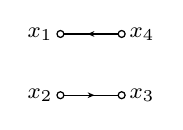
\begin{tikzpicture}[x=0.550cm, y=0.550cm, line width=0.450pt, baseline={([yshift=-0.6ex]0,0)}]
  \draw (0.707,0.707) -- (-0.707,0.707);
  \fill (-0.079,0.707) -- (0.079,0.640) -- (0.028,0.707) -- (0.079,0.775) -- cycle;
  \draw (-0.707,-0.707) -- (0.707,-0.707);
  \fill (0.079,-0.707) -- (-0.079,-0.640) -- (-0.028,-0.707) -- (-0.079,-0.775) -- cycle;
  \draw[fill=white] (-0.707,0.707) circle (0.080);
  \draw[fill=white] (-0.707,-0.707) circle (0.080);
  \draw[fill=white] (0.707,-0.707) circle (0.080);
  \draw[fill=white] (0.707,0.707) circle (0.080);
  \node[font=\footnotesize, inner sep=0pt, anchor=0] at (-0.877,0.707) {$x_{1}$};
  \node[font=\footnotesize, inner sep=0pt, anchor=0] at (-0.877,-0.707) {$x_{2}$};
  \node[font=\footnotesize, inner sep=0pt, anchor=180] at (0.877,-0.707) {$x_{3}$};
  \node[font=\footnotesize, inner sep=0pt, anchor=180] at (0.877,0.707) {$x_{4}$};
\end{tikzpicture}}
\diagramgap
\mbox{$\displaystyle -\,$\,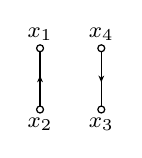
\begin{tikzpicture}[x=0.550cm, y=0.550cm, line width=0.450pt, baseline={([yshift=-0.6ex]0,0)}]
  \draw (-0.707,-0.707) -- (-0.707,0.707);
  \fill (-0.707,0.079) -- (-0.775,-0.079) -- (-0.707,-0.028) -- (-0.640,-0.079) -- cycle;
  \draw (0.707,0.707) -- (0.707,-0.707);
  \fill (0.707,-0.079) -- (0.775,0.079) -- (0.707,0.028) -- (0.640,0.079) -- cycle;
  \draw[fill=white] (-0.707,0.707) circle (0.080);
  \draw[fill=white] (-0.707,-0.707) circle (0.080);
  \draw[fill=white] (0.707,-0.707) circle (0.080);
  \draw[fill=white] (0.707,0.707) circle (0.080);
  \node[font=\footnotesize, inner sep=0pt, anchor=270] at (-0.707,0.877) {$x_{1}$};
  \node[font=\footnotesize, inner sep=0pt, anchor=90] at (-0.707,-0.877) {$x_{2}$};
  \node[font=\footnotesize, inner sep=0pt, anchor=90] at (0.707,-0.877) {$x_{3}$};
  \node[font=\footnotesize, inner sep=0pt, anchor=270] at (0.707,0.877) {$x_{4}$};
\end{tikzpicture}}
